\documentclass{standalone}
\usepackage{tikz}
\begin{document}
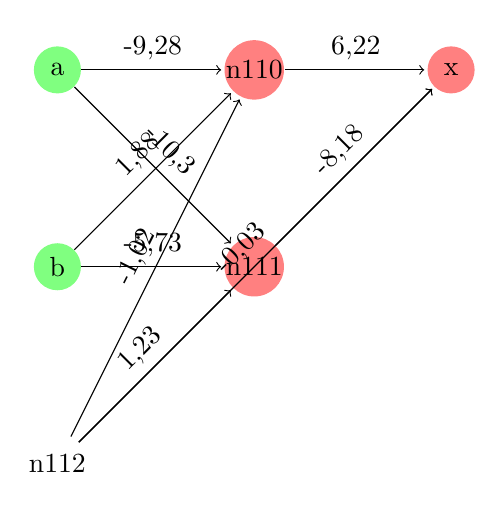
\begin{tikzpicture}[shorten >=1pt,->,draw=black!,node distance=2.5cm]
\tikzstyle{neuron}=[circle,fill=black!25,minimum size=17pt,inner sep=0pt]
\tikzstyle{constant}=[neuron, fill=white!50];
\tikzstyle{sigmoid}=[neuron, fill=red!50];
\tikzstyle{identity}=[neuron, fill=green!50];
\node [identity] (a) {a};
\node [identity,below of=a] (b) {b};
\node [constant,below of=b] (n112) {n112};
\node [sigmoid,right of=a] (n110) {n110};
\node [sigmoid,below of=n110] (n111) {n111};
\node [sigmoid,right of=n110] (x) {x};
\path[every node/.style={sloped,anchor=south,auto=false}]
(n110) edge node {6,22} (x)
(n111) edge node {-8,18} (x)
(a) edge node {-9,28} (n110)
(a) edge node {-10,3} (n111)
(b) edge node {-5,73} (n111)
(b) edge node {1,88} (n110)
(n112) edge node {-0,03} (x)
(n112) edge node {-1,02} (n110)
(n112) edge node {1,23} (n111)
;\end{tikzpicture}
\end{document}